\documentclass[10pt]{article}
\usepackage[margin=1in]{geometry}
\usepackage{amsmath,amssymb}
\usepackage{graphicx}
\usepackage{listings}
\usepackage{xcolor}
\usepackage{tikz}
\usepackage{tcolorbox}
\usepackage{hyperref}

% Colors
\definecolor{codegreen}{rgb}{0,0.6,0}
\definecolor{codegray}{rgb}{0.5,0.5,0.5}
\definecolor{codepurple}{rgb}{0.58,0,0.82}
\definecolor{backcolour}{rgb}{0.95,0.95,0.92}

% Code style
\lstdefinestyle{mystyle}{
    backgroundcolor=\color{backcolour},   
    commentstyle=\color{codegreen},
    keywordstyle=\color{magenta},
    numberstyle=\tiny\color{codegray},
    stringstyle=\color{codepurple},
    basicstyle=\ttfamily\footnotesize,
    breakatwhitespace=false,         
    breaklines=true,                 
    captionpos=b,                    
    keepspaces=true,                 
    numbers=left,                    
    numbersep=5pt,                  
    showspaces=false,                
    showstringspaces=false,
    showtabs=false,                  
    tabsize=2
}
\lstset{style=mystyle}

% Custom commands
\newcommand{\checkpoint}[1]{
    \begin{tcolorbox}[colback=yellow!10!white,colframe=yellow!75!black,title=Checkpoint]
    #1
    \end{tcolorbox}
}
\newcommand{\activity}[1]{
    \begin{tcolorbox}[colback=blue!5!white,colframe=blue!75!black,title=Activity]
    #1
    \end{tcolorbox}
}
\newcommand{\realworld}[1]{
    \begin{tcolorbox}[colback=green!5!white,colframe=green!75!black,title=Real World Example]
    #1
    \end{tcolorbox}
}

\title{Week 5: Transformers - The Architecture Behind ChatGPT\\
\large Simplified BSc Handout with Visual Learning}
\date{}

\begin{document}
\maketitle

\section*{Today's Journey}
Imagine you're in a classroom where everyone can talk to everyone else at the same time, instead of passing notes one by one. That's the transformer revolution!

\hrule
\vspace{1em}

\section{Part 1: Why Transformers? The Problem with Sequential Processing}

\subsection{The Telephone Game Problem}

\activity{
Play telephone with this sentence: "The quick brown fox jumps over the lazy dog"

Person 1 → Person 2 → Person 3 → ... → Person 10

What happens to the message?
}

This is how RNNs work - information degrades as it passes through the network sequentially.

\subsection{The Parallel Processing Solution}

\realworld{
\textbf{RNN (Sequential)}: Like reading a book one word at a time with your finger
\textbf{Transformer (Parallel)}: Like seeing the whole page at once
}

\begin{center}
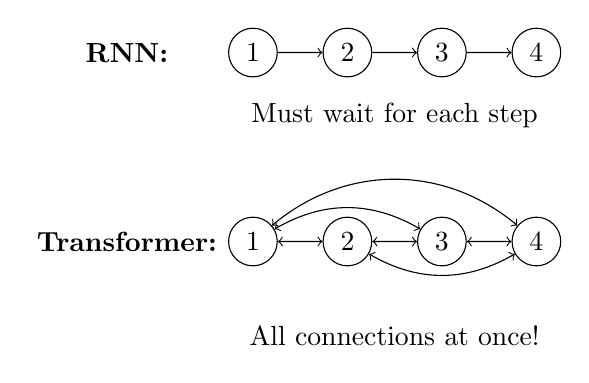
\begin{tikzpicture}[scale=0.8]
    % RNN
    \node at (0, 2) {\textbf{RNN:}};
    \node[circle,draw] (r1) at (2,2) {1};
    \node[circle,draw] (r2) at (3.5,2) {2};
    \node[circle,draw] (r3) at (5,2) {3};
    \node[circle,draw] (r4) at (6.5,2) {4};
    \draw[->] (r1) -- (r2);
    \draw[->] (r2) -- (r3);
    \draw[->] (r3) -- (r4);
    \node at (4.25, 1) {Must wait for each step};
    
    % Transformer
    \node at (0, -1) {\textbf{Transformer:}};
    \node[circle,draw] (t1) at (2,-1) {1};
    \node[circle,draw] (t2) at (3.5,-1) {2};
    \node[circle,draw] (t3) at (5,-1) {3};
    \node[circle,draw] (t4) at (6.5,-1) {4};
    \draw[<->] (t1) -- (t2);
    \draw[<->] (t1) to[bend left=30] (t3);
    \draw[<->] (t1) to[bend left=40] (t4);
    \draw[<->] (t2) -- (t3);
    \draw[<->] (t2) to[bend right=30] (t4);
    \draw[<->] (t3) -- (t4);
    \node at (4.25, -2.5) {All connections at once!};
\end{tikzpicture}
\end{center}

\checkpoint{
\textbf{Key Insight}: Transformers process all words simultaneously, making them much faster on modern hardware!
}

\section{Part 2: Self-Attention - The Core Innovation}

\subsection{The Attention Mechanism Explained Simply}

Think of attention like a \textbf{spotlight in a theater}:
\begin{itemize}
    \item Each word is an actor on stage
    \item Each actor has a spotlight they control
    \item They can shine their spotlight on other actors (or themselves)
    \item The brightness shows how much they're paying attention
\end{itemize}

\subsection{The Three Roles: Query, Key, Value}

\realworld{
Imagine a library:
\begin{itemize}
    \item \textbf{Query}: "I'm looking for books about cats"
    \item \textbf{Key}: Each book's catalog card
    \item \textbf{Value}: The actual book content
\end{itemize}
You compare your query to all keys, then take the values of matching books!
}

\subsection{Visual Example: How "cat" Attends to Other Words}

\begin{center}
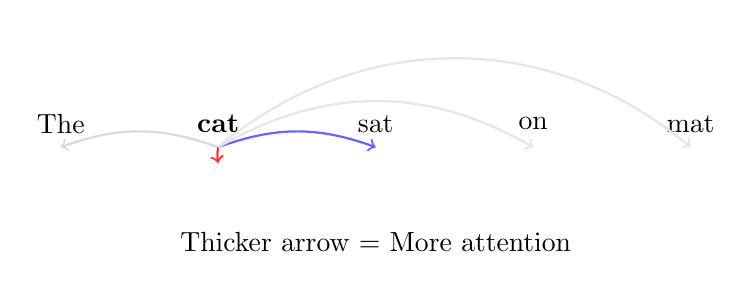
\begin{tikzpicture}[scale=1]
    \node at (0,0) {The};
    \node at (2,0) {\textbf{cat}};
    \node at (4,0) {sat};
    \node at (6,0) {on};
    \node at (8,0) {mat};
    
    % Attention weights (visual)
    \draw[->, thick, color=gray!30] (2,-0.3) to[bend right=20] (0,-0.3);
    \draw[->, thick, color=red!80] (2,-0.3) to[bend right=10] (2,-0.5);
    \draw[->, thick, color=blue!60] (2,-0.3) to[bend left=20] (4,-0.3);
    \draw[->, thick, color=gray!20] (2,-0.3) to[bend left=30] (6,-0.3);
    \draw[->, thick, color=gray!20] (2,-0.3) to[bend left=40] (8,-0.3);
    
    \node at (4,-1.5) {Thicker arrow = More attention};
\end{tikzpicture}
\end{center}

\activity{
For the sentence "The student loves pizza", draw attention arrows from "loves" to each word. Which words should get the most attention?
}

\section{Part 3: Multi-Head Attention - Different Perspectives}

\subsection{Why Multiple Heads?}

\realworld{
Like having multiple cameras filming a scene:
\begin{itemize}
    \item Camera 1: Focuses on the main actor (subject)
    \item Camera 2: Captures the action (verb)
    \item Camera 3: Shows the setting (context)
    \item Camera 4: Tracks emotions (sentiment)
\end{itemize}
Each "head" captures different relationships!
}

\subsection{Visual: 4 Heads Looking at "bank"}

\begin{center}
\begin{tabular}{|l|l|l|}
\hline
\textbf{Head} & \textbf{Focus} & \textbf{Attends to} \\
\hline
Head 1 & Syntax & "The" (determiner) \\
Head 2 & Meaning & "river" (context) \\
Head 3 & Position & nearby words \\
Head 4 & Topic & "water", "flow" \\
\hline
\end{tabular}
\end{center}

\checkpoint{
Each head learns to look for different patterns. Together, they understand language from multiple angles!
}

\section{Part 4: Positional Encoding - Teaching Order}

\subsection{The Position Problem}

Without position information:
\begin{itemize}
    \item "Cat chased mouse" = same as "Mouse chased cat"
    \item "John loves Mary" = same as "Mary loves John"
\end{itemize}

\activity{
Write two sentences using the same words but different order, where the meaning completely changes:

1. \_\_\_\_\_\_\_\_\_\_\_\_\_\_\_\_\_\_\_\_\_\_\_\_\_

2. \_\_\_\_\_\_\_\_\_\_\_\_\_\_\_\_\_\_\_\_\_\_\_\_\_
}

\subsection{The Sine Wave Solution}

\realworld{
Like giving each word a unique "address":
\begin{itemize}
    \item Position 1: [0.84, 0.54, 0.00, 1.00, ...]
    \item Position 2: [0.91, 0.42, 0.84, 0.54, ...]
    \item Position 3: [0.14, -0.99, 0.91, 0.42, ...]
\end{itemize}
Each position has a unique pattern, like a fingerprint!
}

\section{Part 5: Building a Complete Transformer}

\subsection{The Layer Cake Architecture}

\begin{center}
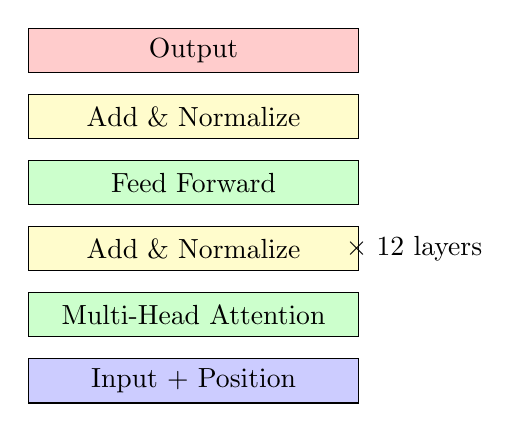
\begin{tikzpicture}[scale=0.7]
    % Input
    \draw[fill=blue!20] (0,0) rectangle (6,0.8);
    \node at (3,0.4) {Input + Position};
    
    % Layer 1
    \draw[fill=green!20] (0,1.2) rectangle (6,2);
    \node at (3,1.6) {Multi-Head Attention};
    
    \draw[fill=yellow!20] (0,2.4) rectangle (6,3.2);
    \node at (3,2.8) {Add \& Normalize};
    
    \draw[fill=green!20] (0,3.6) rectangle (6,4.4);
    \node at (3,4) {Feed Forward};
    
    \draw[fill=yellow!20] (0,4.8) rectangle (6,5.6);
    \node at (3,5.2) {Add \& Normalize};
    
    % Stack indicator
    \node at (7,2.8) {$\times$ 12 layers};
    
    % Output
    \draw[fill=red!20] (0,6) rectangle (6,6.8);
    \node at (3,6.4) {Output};
\end{tikzpicture}
\end{center}

\checkpoint{
Like a layer cake, each layer adds more understanding. GPT-3 has 96 layers!
}

\subsection{Residual Connections - Information Highways}

\realworld{
Like having both stairs AND an elevator in a building:
\begin{itemize}
    \item Stairs = Going through the transformation
    \item Elevator = Direct connection (residual)
\end{itemize}
Information can take either path!
}

\section{Part 6: Hands-On Code Understanding}

\subsection{Simplified Attention in Python}

\begin{lstlisting}[language=Python]
# Simplified self-attention (conceptual)
def attention(sentence):
    words = sentence.split()
    attention_scores = {}
    
    for word1 in words:
        scores_for_word1 = {}
        for word2 in words:
            # How relevant is word2 to word1?
            score = calculate_relevance(word1, word2)
            scores_for_word1[word2] = score
        
        # Normalize scores to sum to 1
        total = sum(scores_for_word1.values())
        for word2 in scores_for_word1:
            scores_for_word1[word2] /= total
        
        attention_scores[word1] = scores_for_word1
    
    return attention_scores

# Example usage
result = attention("The cat sat")
# result["cat"] might be: {"The": 0.2, "cat": 0.3, "sat": 0.5}
\end{lstlisting}

\activity{
Trace through this code with "I love pizza". What would result["love"] contain?
}

\section{Part 7: Real-World Applications}

\subsection{Transformers Everywhere!}

\begin{center}
\begin{tabular}{|l|l|l|}
\hline
\textbf{Application} & \textbf{Model} & \textbf{What it Does} \\
\hline
Chat & ChatGPT & Conversations \\
Translation & Google Translate & 100+ languages \\
Code & GitHub Copilot & Writes code \\
Images & DALL-E & Creates pictures \\
Science & AlphaFold & Protein folding \\
\hline
\end{tabular}
\end{center}

\realworld{
When you use autocomplete on your phone, that's a tiny transformer running locally!
}

\section{Part 8: Practice Problems}

\subsection{Problem 1: Attention Weights}

Given the sentence "Dogs love treats", fill in reasonable attention weights:

\begin{center}
\begin{tabular}{|l|c|c|c|}
\hline
\textbf{From $\downarrow$ To $\rightarrow$} & Dogs & love & treats \\
\hline
Dogs & 0.5 & \_\_\_ & \_\_\_ \\
love & \_\_\_ & 0.2 & \_\_\_ \\
treats & \_\_\_ & \_\_\_ & 0.4 \\
\hline
\end{tabular}
\end{center}

Remember: Each row must sum to 1.0!

\subsection{Problem 2: Parallelization}

Calculate the speedup:
\begin{itemize}
    \item Sentence length: 50 words
    \item RNN: Processes 1 word per time step
    \item Transformer: Processes all words at once
\end{itemize}

Time for RNN: \_\_\_\_ steps
Time for Transformer: \_\_\_\_ step(s)
Speedup: \_\_\_\_ times faster

\subsection{Problem 3: Design Challenge}

Design a 2-head attention system for understanding "Time flies like an arrow":
\begin{itemize}
    \item Head 1 focuses on: \_\_\_\_\_\_\_\_\_\_\_\_\_
    \item Head 2 focuses on: \_\_\_\_\_\_\_\_\_\_\_\_\_
\end{itemize}

\section{Key Takeaways}

\checkpoint{
Remember these 5 key points:
\begin{enumerate}
    \item Transformers process all words \textbf{in parallel}
    \item Self-attention creates \textbf{direct connections} between all words
    \item Multiple heads capture \textbf{different relationships}
    \item Position encoding tells the model about \textbf{word order}
    \item This architecture powers \textbf{ChatGPT} and modern AI!
\end{enumerate}
}

\section{Bonus: Fun Facts}

\begin{itemize}
    \item The transformer paper has been cited over 100,000 times!
    \item GPT-3 would take 355 years to train on a single GPU
    \item Transformers can work with images, music, and even DNA sequences
    \item The name comes from "transforming" one sequence to another
    \item The original transformer was trained for translation in just 3.5 days
\end{itemize}

\hrule
\vspace{1em}

\section*{Next Steps}

\begin{enumerate}
    \item Try the Jupyter notebook to build your own transformer
    \item Experiment with attention visualizations
    \item Read "Attention Is All You Need" paper (challenge yourself!)
\end{enumerate}

\realworld{
You now understand the architecture that powers ChatGPT, BERT, and almost every modern NLP system. That's huge!
}

\end{document}